Ziel dieser Arbeit wird es im Grunde sein, Donuts besser zu verstehen. Fachlich wird ein Donut-\-ähn\-liches Gebilde als \emph{Torus} (plural: \emph{Tori}) bezeichnet. Wir wollen herausfinden, wann zwei Tori auf eine gewisse Art \enquote{sehr ähnlich} zueinander sind. 

Tori werden in der Kryptographie verwendet und dort spielt genau diese \enquote{Ähnlichkeit} eine Rolle. Innermathematisch finden sich Anwendungen im Bereich der algebraischen Geometrie.

Unsere Analyse basiert dabei anschaulich auf folgender \enquote{Bastelanleitung} für Donuts bzw. Tori:
\begin{Bastelanleitung}
 \begin{enumerate}[1.]
	\item Forme eine Röhre aus einem Blatt Papier. Das heißt: Verklebe die zwei langen Kanten des Papieres miteinander.
	\item Forme jetzt einen Ring aus dieser Röhre. Das heißt: Verklebe die beiden kurzen Kanten miteinander.
\end{enumerate}
\begin{center}
 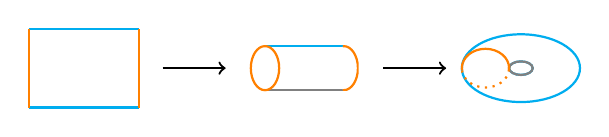
\begin{tikzpicture}[thick]
	\fill[white] (0,0) rectangle (1.4,1);
	\draw[cyan] (0,0) -- (1.4,0);
	\draw[cyan] (0,1) -- (1.4,1);
	\draw[orange] (0,0) -- (0,1);
	\draw[orange] (1.4,0) -- (1.4,1);
	%Mitte
	\begin{scope}[xshift=3cm, yshift = 0.5cm]
		\fill[white] (0,-0.28) rectangle (1,0.28);
		\draw[cyan] (0,0.28cm) -- (1,0.28cm);
		\draw[gray] (0,-0.28cm) -- (1,-0.28cm);
		\filldraw[fill=white, draw=orange] (0,0) circle[x radius= 0.18cm, y radius=0.28cm, ];
		\begin{scope}[xshift=1cm]
			\clip (-0.01cm,-0.29cm) rectangle (0.19cm, 0.29cm);
			\draw[fill=white, draw=orange] (0,0) circle[x radius= 0.18cm, y radius=0.28cm];
		\end{scope}
		%Donut
		\begin{scope}[xshift=3.25cm, scale=1.5]
			\begin{scope}[yscale = cos(55)]
				\draw[even odd rule, draw=cyan, fill=white] 
				(0,0) circle [radius = 0.5cm]
				(0,0) circle [radius=0.1cm];
				\draw[gray] (0,0) circle [radius=0.1cm];
				%\draw[draw=gray, 
				%fill=LimeGreen!20!white
				%] 
			\end{scope}
			\begin{scope}[yscale = sin(55)]
				\clip (-0.51cm,-0.01cm) rectangle (0.01cm, 0.29cm);
				\draw[orange] (-0.3cm, 0) circle (0.2cm);
			\end{scope}
			\begin{scope}[yscale = sin(55)]
				\clip (-0.51cm,0.01cm) rectangle (0.01cm, -0.29cm);
				\draw[dotted, orange] (-0.3cm, 0) circle (0.2cm);
			\end{scope}
		\end{scope}
	\end{scope}
		\draw[->] (1.7,0.5) -- (2.5,0.5);
		\draw[->] (4.5,0.5) -- (5.3,0.5);
 \end{tikzpicture}
\end{center}
\end{Bastelanleitung}

Zugegebenermaßen wird das Ergebnis dieser Anleitung ein nur mehr oder weniger hübscher Torus sein. Das Prinzip kann man allerdings genau so in rigorose Fachmathematik übersetzen. 

Das Blatt Papier -- allgemein ein beliebiges Parallelogramm -- kann als eine Teilmenge in der Ebene aufgefasst werden; der Torus als eine Mannigfaltigkeit. 

Will man mathematische Objekte im Allgemeinen miteinander vergleichen, so betrachtet man meist Abbildungen zwischen ihnen; in unserem Fall Abbildungen zwischen Tori, also zwischen Mannigfaltigkeiten. Betrachtet man stetige Abbildungen, sind alle Tori isomorph bzw. homöomorph zueinander. Dasselbe gilt für differenzierbare Abbildungen, wenn man den Torus mit einer differenzierbaren Struktur ausstattet. Interessanter wird es, wenn man diesen mit einer sogenannten \emph{komplexen Struktur} ausstattet.

Ganz analog zum reellen Fall kann man nämlich \emph{komplexe Mannigfaltigkeiten} und \emph{holomorphe Abbildungen} zwischen diesen definieren. Der Torus wird dabei zu einer komplexen Mannigfaltigkeit, wenn man die euklidische Ebene \(\R^2 \cong \C\) mit der komplexen Ebene identifiziert.


Da Holomorphie eine wesentlich stärkere Eigenschaft als Differenzierbarkeit ist, gibt es in diesem Fall Tori, die eben nicht isomorph bzw. \emph{biholomorph} zueineander sind. Die vorliegende Arbeit soll also folgende Fragestellung beantworten:
\begin{marked}
	\begin{center}
		\emph{Wann genau gibt es eine biholomorphe Abbildung zwischen zwei komplexen Tori?}
	\end{center}
\end{marked}
Um diese Frage zu beantworten, brauchen wir im Grunde drei Zutaten:
\begin{enumerate}[1.]
	\item Begriff der \emph{komplexen Quotientenmannigfaltigkeit}.
	\item Prinzip des \emph{Hochhebens} von Abbildungen.
	\item \emph{Satz} aus der Funktionentheorie über ganze \emph{biholomorphe Funktionen}.
\end{enumerate}

Wir werden uns erst mit Mannigfaltigkeiten beschäftigen. Dabei wird der Begriff der \emph{Quotientenmannigfaltigkeit} erarbeitet. Dieser präzisiert das anfangs beschriebene \enquote{Verkleben} der Papierseiten.
Daraufhin sollen \emph{kom\-plexe Mannigfaltigkeiten} in beliebigen Dimensionen eingeführt werden. Der Begriff der Holomorphie wird zu diesem Zweck auf mehrere Veränderliche verallgemeinert. 

Im darauffolgenden Kapitel werden für uns relevante Begriffe der algebraischen Topologie erarbeitet. Zentral für den Beweis des Resultats am Ende der Arbeit wird das sogenannte \emph{Hochheben} von Wegen beziehungsweise Abbildungen sein.
